\chapter{Smart Grid}\label{chap:sg}
The Smart Grid  is a new concept of grid which introduces new technologies into the traditional power system. They enable power grids to become more efficient, integrate other sources of energy rather than traditional ones, and  they increase the overall management performance by using modern information technologies. The SG is capable of delivering power in more efficient way and respond to a wide variety of condition and events \cite{journals/comsur/FangMXY12}. Although there are no SGs fully implemented, there are several SG pilot projects  show that the new generation grid pose new opportunities and challenges to both consumers and producers. \\
There are several definitions for the SG among the literature. For example \cite{journals/comsur/FangMXY12} states that  "\textit{SG can be regarded as an electric system that uses information, two-way and cyber-secure communication technologies and computational intelligence in an integrated fashion to achieve a clean, safe, secure, reliable, resilient, efficient and sustainable system}".\cite{conf/isgt/GhoshPR13} considers the SG as "\textit{a platform that embraces several multidisciplinary concepts towards computerization of electrical power grids}". The common concept over the literature is that SG main goal is to integrate several components, traditional and new, to achieve better performance, interoperability, energy management and sustainability in long term. \\
SG creates an environment that introduces a convergence between the infrastructure of generation, transmission, distribution, energy, information technology and digital communication infrastructure that enables the exchange of information and control action among the various segments of the power grid.\\
As it is possible to notice, these integration means that the SG itself is a very complicated system. Achieving the mentioned goals is a complex task. Due to its variety of problems and challenges, most of the proposed solution and studies regarding the SG focus in some specific aspects. 
An interesting table that presents a comparison between the traditional grid and the SG is presented in \cite{journals/comsur/FangMXY12}:
\begin{figure}[h]
\centering
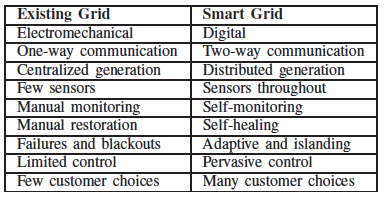
\includegraphics[width=0.5\textwidth]{/Users/rafaelremondes/UM/MEI/Thesis/DistributedAggregationAlgortihmsSM/Writing/Images/differencesTraditionalSmart}
\caption{\label{fig:comparisonOldNew} Brief Comparison Between the Existing Grid and the Smart Grid}
\end{figure}

\section{Smart Grid Model}
 The  SG  proposes a new model to the power grid where consumers are no longer passive actors in the grid, but prosumers(insert quote) that can both consume and produce energy in small quantities thanks to the new renewable energy sources, plus the introduction of ICT that means new actors that are now present in the grid, enabling new features into the traditional ones.\\
 Typically, the components in a power grid go one way, in the in SG  all the flows of electricity and information go two-ways.  These new features enable the operations to become  faster and more accurate and the interactions between them  are increased resulting that, in the future, everything that happens in the grid can be monitored almost in real time.\\
 In am ideal scenario, the SG's new vision, states that a specific component of the grid, such as a household, can both receive energy from the global grid and in the next moment can disconnect from it and become self-sustainable. \\
There are several visions and models proposed to the SG. One of the more general and accepted model, based on this vision of actors and their interactions, is  the NIST report \cite{government2011nist} which proposes a conceptual model providing the main actors towards the SG.
\begin{figure}[h]
\centering
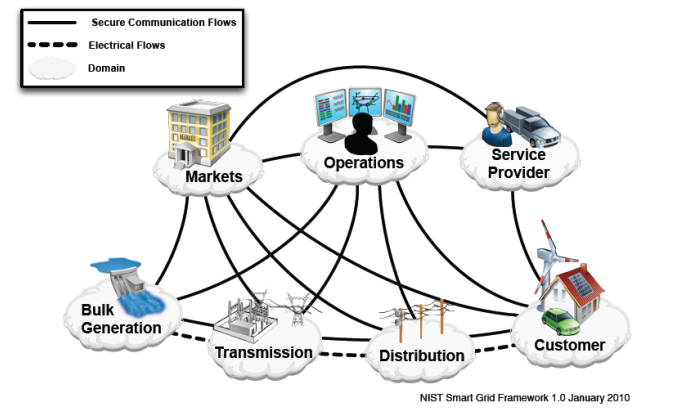
\includegraphics[width=0.75\textwidth]{/Users/rafaelremondes/UM/MEI/Thesis/DistributedAggregationAlgortihmsSM/Writing/Images/NIST_model}
\caption{\label{fig:NIST_model} NIST Conceptual Model for SG}
\end{figure}
Costumers, the end users of electricity, Markets, Service Providers, Electricity Companies, Operations, Managers of the Movement of electricity, Bulk Generation, Generation Centers, Transmission and Distribution of energy. 
In \cite{journals/comsur/FangMXY12} it is provided a more technical approach where the SG is separated into three major subsystems:
\begin{itemize}
\item \textit{Smart infrastructure system} embraces the energy subsystem, information subsystem and communication infrastructure subsystem. The energy subsystem is responsible for advanced electricity generation, delivery and consumption. The information subsystems are responsible for information metering, monitoring and management in the context of the SG. Finally, the communication subsystem is responsible for the communication among the various components and also its connectivity.   
\item \textit{Smart management system} Provides advanced management and control services and functionalities, \cite{journals/comsur/FangMXY12} considers this system the key reason why SG can revolutionize the grid.  Most of the new grid goals are related to energy efficiency improvement, supply and demand balance, emission control etc. and it is the scope of problems the management systems tries to resolve.
\item \textit{Smart protection system} Provides advanced grid reliability analysis, failure protection, security and privacy protection services.
 \end{itemize}
Smart Grids are about improving the current power grid in therms of reliability, energy efficiency and costs  while providing a better and more flexibly service to the costumers. These improvements are made possible with the integration of ICT into the power grid, leading to a opportunity for the dawn of new software applications. In \cite{Andrea} it is stated that Service Oriented Architectures represent the type of software architecture that satisfies the characteristics needed for a SG software: capable of sustaining a set of systems and applications that are diverse, highly distributed and with constrains for security and timing.  In  \cite{Andrea} it is provided an overall picture that show that show the interaction between these type of software and the physical infrastructure.
\begin{figure}[h]
\centering
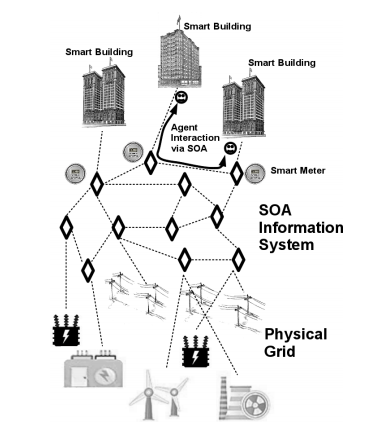
\includegraphics[width=0.75\textwidth]{/Users/rafaelremondes/UM/MEI/Thesis/DistributedAggregationAlgortihmsSM/Writing/Images/interaction}
\caption{\label{fig:Interaction_model} Smart grid physical and information infrastructure}
\end{figure}

\section{Smart Grid Communication}
The most important question regarding the communication is "\textit{ what network and communication should be used}"\cite{journals/comsur/FangMXY12}? Since there is no standard communication system in SG, several communication solutions were proposed divided into wired and wireless communication.\\
Wired solutions are normally more costly to implement than Wireless, mainly because of the need, in some cases, to install or deploy from zero a physical infrastructure like cables to link the components in order to enable communication.  Wireless communication can be a better option in terms of cost, time to deploy and furthermore they are normally more suitable for remote end applications \cite{parikh2010opportunities}. However, they lack of some performance compared to wired solutions, specially in speed. Also, the costs of deploying an wired communication infrastructure can be reduced if they are implemented in the existing infrastructure, case of power line communication that use the power cables.\\
There are several wireless possibilities for communication.\\
\begin{itemize}
  \item \textit{Wireless Mesh Network} (WMN) is a communication network made up for radio nodes organized in a mesh topology\cite{journals/comsur/FangMXY12}. It increases reliability and automatic network connectivity, has large coverage and high data rate.
\item \textit{Cellular Communication Systems}  GSM and 3G. Useful in case of low computation power devices such as the meters. It is quick and low-cost to obtain data communications coverage over a large geographic area \cite{akyol2010survey}. There several solutions that use a Short Message Service communication to send the meters data.
\item \textit{Wireless Communication based on 802.15.4} ZigBee is a wireless communication that is recommended to be used in SG considering the IEEE 802.15.4 protocol stack\cite{parikh2010opportunities}. ZigBee is designed for radio-frequency applications that require low data rate, long battery life, and secure networking. Selected as the communication technology for the smart metering devices\cite{farhangi2010path} because it provides a standardized platform for exchanging data between smart metering devices and appliances located on costumer  premises\cite{journals/comsur/FangMXY12}.  WiMax, WirelessHART and ISA100.11a are other examples of wireless communications based on the IEEE 802.15.4 protocol.
\end{itemize}
Other examples of wireless communication are satellite cognitive radio and  microwave communications.
Fiber-optic Communications and Power-line Communications are some of the wired communication possibilities. Power-line communication has the advantage of being already installed, so the cost of deployment is less expensive than other wired solutions. Fiber-Optic has also the advantage of being fast  but it can be more expensive to deploy because of the need to implement from zero in an infrastructure that lacks cables with that sort of technology.\\



%%%%%SMART METERS-----------------%

\section{Smart Information SubSystem}\label{sec:sginformation}
This part of the SG refers to the whole information that is collected by sensing the consumers consumption and its management . The data collected is often used for billing, grid status monitoring and user appliance control \cite{journals/comsur/FangMXY12}. It is aggregated and collected, afterwards \textit{smart management} is ideally performed on the data.\\
An important concept in the information subsystem  is the \textit{Smart Metering} and the Smart Metering System or Automatic Meter Reading \nom{AMR}{Automatic Meter Reading}. This system is responsible for collect the data from the measurements that are performed by the SMs.\\
Other part of the Smart Information SubSystem is the \textit{Smart Monitoring and Measurement} which can be approached by either \textit{sensors} or \textit{phasor measurement units}(PMU). \textit{Sensors} are used for detecting failures, tower collapses, hotspots and extreme mechanical conditions. They can also provide real-time diagnose of the grid status. PMU's are devices that measure the electrical waves on a electrical grid to determinate the health  of the system. These systems collect information regarding the status of the grid in order to monitor it and detect failures and outages.\\
 The Smart Metering Systems  only collects data from SM's and it only embraces the management of that data.The management refers to the whole information analysis and modeling, integration and optimization.In this specific part of SG there are several areas of research that represent a new set of opportunities.

\subsection{AMR and AMI}\label{subsec:amrami}
As referred in this document, the smart metering system is composed by smart meters that sense the energy consumption and send  their data to a Gateway or a Data Collector. It can also be defined as AMR or  \nom{AMI}{Automated Metering Infrastructure}. In \cite{journals/spm/ErkinTLP13}, the AMR is described in more detailed as an "\textit{technology of automatically collecting diagnostic, consumption and status data from energy metering devices and transferring that data to a database for billing troubleshooting and analyzing}".\\
 The Automated Metering Infrastructure is a more sophisticated version of the traditional AMR, it provides two-way communication, enabling a more sophisticated control of a smart meter behavior. Therefore, all of the meter information is available in real time, allowing improved system operations and  costumer power demand management\cite{journals/spm/ErkinTLP13}.  AMI has also the ability of reconfigure from communication failures, perform outage management and reporting, service connect and disconnect and it also enables time stamping of meter data \cite{hart2008using}. AMI is built upon AMR. \\
Current SM enable two-way communication, an important part of the benefits that come from the usage of this new meters, comes from two-way communication, also two-way communication is not only important for behavior control and outage detection, it enables the realization and implementation of in-network algorithms. Now it is more correct to assume that every AMR has an AMI built upon it enabling two-way communication.\\
In the pilot projects studied, a smart metering system is, of course, composed by the smart meters. The common part is that in a  pre-defined period of time, the devices send the consumption data. In projects, a cloud based service is used for the  SM to send the data . In other cases, substations that work as data collectors are used to concentrate  the consumption information from the SMs connected to it, usually a whole neighborhood, afterwards, the data from the substations is sent to a data center. In small SG, there is no central data center. The substations communicate with each other.\\ 



\subsection{Smart Meters}
Smart meters are devices that sense the energy consumption. They are installed in the costumer side,  households or in  industrial facilities, depending on the costumer nature. Playing a major role in the information subsystem, smart meters present several number of challenges in sensing and analyzing\cite{journals/spm/ErkinTLP13}. SMs, more specifically, the Smart Mettering System has also the denomination of AMR(Automatic Meter Reading). In \cite{khalifa2011survey} the AMR is referred as the technology whose goal is to help collect the meter measurement automatically and possibly send commands to the meters.\\
As referred in the previous section, the main function of a smart meter, and all meters, is sense the consumption in the costumer side. The feature of sending their data, allocate and aggregate the information that comes from many meters allows a company to remotely read the consumers' consumption at each household, without the need to actually go to the premises and without notifying the costumers\cite{Ericsson_2}. Jorge Vasconcelos \cite{RePEc:erp:euirsc:p0193} enlightens in his work the potential benefits of the smart meters, for  example, the potential benefits for customers are customer awareness and energy saving, more accurate meter reading, billing, better service quality, greater tariff variety and flexibility, improved conditions for vulnerable customers, easier comparability of offers and it is easier to change supplier. \cite{khalifa2011survey} states some benefits of the smart metering system: Real time pricing, power quality measurement, automated Billing, Load management,, Remote Connect/Disconnect, Outage notification and Bundling with water and gas.\\
Privacy and security are important concerns when dealing with the sensed information. There are many privacy issues considering that external parties access the consumer energy consumption. Some are authorized parties, but there is a risk of an unauthorized access of this data, leaving to some security and privacy dangers. For example, by analyzing the data, one could determinate which devices are plugged in at some specific time, giving for example information about if there is people in home or note. Many pieces of work propose solution to securely store this sensible information. Although privacy and security are out of the scope of this work, it is important to mention this point.\\

\subsection{Smart Grid Projects}
So far there aren't standards to realize the Smart Grid, as it was aforementioned, not even a complete and specific definition about what is a Smart Grid. Even without a specific definition regarding the standard model and communication, there  are common concepts that are well accepted and visions that are transversal . The introduction of communication and information technology into the grid, the idea of a consumer that is not only a consumer but also a small producer that can supply the grid and itself with electrical energy, the remote control of the components like electrical cable and station and more, are ideas that seem to be features that all future SG will have. In order to understand how it is currently the status of the SG and the directions it will take in the future, we analyze several pilot projects and companies that are know a days trying to implement the new grid.
\subsubsection{Opower 4}
Opower\cite{website:opower} iis a company that promises to help costumers to reduce their energy consumption. They provide a cloud based service to gather data regarding the costumers information about their energy consumption, and using big data and behavioral science they provide reports to the costumer with their consumption history in the time period that report is about. Also, the reports give tips and advices where the consumer can reduce the energy consumption, and therefore, reduce the energy bill.\\
One of the version of the promised platform, one of the most recent, is called Opower 4. Opower 4 works as a service platform, is a \textit{Software as a Service} platform. The model is like the general model for the SG Information subsystem described in section \ref{chap:sg}. Households using this services have a smart meter installed, every 15 minutes, the device send the data to a cloud through a cloud based service. The collection of the data is only made in one point, in a Data Center that concentrates all data. There is no reference regarding the number of data centers that the company uses. Big Data is performed in the data. Mainly, as it was stated, the platform exists for billing proposes and to raise awareness in the costumers so that they reduce their consumption with reports that have statistics of each household. For example, one costumer comparison with the neighborhood and what devices are consuming more or less.
\subsection{DEHEMS Project}
The DEHEMS project \cite{website:dehems}t is an infrastructure that reasons about the household's energy behavior and tests various persuasive techniques effectiveness. The system receives energy information from several sensing devices, including the ones that sense electrical consumption. The special feature about the DEHEMS project is that it uses Informix TimeSeries \cite{website:informix} that is a built­in feature of Informix, a database type of IBM, that adds support for managing time series (time­stamped) data, this feature is specially important in the management of data regarding the reading of the meter.\\
This project operates in the distribution grid. The model also includes de household, where several sensors are installed, not only for electricity, but also for gas and water. Each sensor, with a 433Mhz Radio, takes reading every 6 seconds and sends it to a DEHEMS Gateway that aggregates all the information about the house. The data of all the Gateways is concentrated in a Informix database so that big data operations can be performed on it.\\The goal of this project is the same as the aforementioned project, raise awareness in the costumers by generating statistics abou each household consumption(CO2 emissions, cost of the energy, history of consumption and comparison with the other consumers) and send it to the consumer.
\subsubsection{Pecan Street Project}
The Pecan Street Project\cite{website:pecan} is a research project / is researching a project?? in Smart Grids by Pecan Street Inc., a University of Texas­based research organization. Started in Austin an then expanded to other cities and states. The focus of the research is mainly in the information subsystem of Smart Grid. One of the project goals is to understand how to lower the carbon emissions by learning how energy is being used among homes. But understanding the “how†is only half of the challenge: Pecan Street also seeks to understand what homeowners need in order to manage their energy use.\\
As the other, it operates in the distribution grid and it works in a similar way as the DEHEMS project. In each house, there are several sensors installed to sense the consumption in each device, for example the Air Condition System. The sensors send their data every 2 seconds to the gateway and then to the smart meter every 15s, the meter sends the collected information from the gateway to a data center every 15 minutes. In the gateway it is performed an estimated average of all devices connected to a sensor. The consumption data is in the end used for statistical analysis to produce results about the consumer energy consumption. With this information, the Pecan Street Project staff pretends to lead their costumers to use their energy more efficiently.
\subsubsection{Smart Meter Data Stream in the Cloud}
This is a solution proposed to handle the SM data in a distribution electrical grid which is in
\cite{lohrmann2011processing} for real time pricing. The simulation considers a set of 1 million meters connect via TCP/IP to a data center/Cloud. Every second, each SM sends a package containing information about the electrical consumption of an household. The cloud model is composed by layers. Since every moment a new package arrives, it is like a stream, so several stream tasks are created in the lowest layer to handle the incoming data. In the upper level, within the cloud, aggregation tasks are created and they work in parallel to handle the information that comes from the lower level, the stream tasks. As the traffic increases or decreases, more aggregation tasks are created or deleted accordingly. In the paper simulation, 2 aggregation task were created. In the highest lawyer there is one real time pricing task that has the role of updating the energy price according to the amount of the energy consumed.\\
This paper offers a solution to handle smart meters data to provide a real­time pricing policy to balance the
demand of energy and also to continuously monitoring of the meter, mainly to prevent outages and blackouts during peak time.
\subsubsection{Inovgrid/InovCity}Inovgrid\cite{matos2013inovgrid} is a project powered by EDP, Energias de Portugal, that pretends to modernize the portuguese electrical grid, more specifically, the distribution grid, in other words, the project aims to transform the traditional grid into a smart grid by adding information and communication technology. This is still a pilot project, there is no mass scale attempts yet to fully implement.So far, there is only a pilot project called the InovCity in the city of Évora that consists of a smart grid small experiment, with the installation of several smart meters and sensors in some of Évora households. \\
In further detail, the InovCity model can be explained by dividing the grid into three smaller networks: a Home Area Network(HAN), a network in each house, whereas each device has a sensor that communicates with the smart meter installed in the house. In the set of devices that composes the HAN, electrical vehicles are also included.
Local Area Network, a set of households, a neighborhood connect to a DTC/substation that communicates through the electrical cables, PLC Prime and LMS protocol. Finally, the wide area network that embraces all the other minor networks\\
In terms of number, in InovCity 300 000 Smart Meters and 300 DTC/Substations were installed. The Smart Meteres communicate the consumption of an household every 15 minutes to a Substation which therefore communicates to other substation and finally to a central facility. Each substation has the capability of performing data analysis and process data function, so, depending on the type of analysis, the substation can perform it locally. Basically, the whole collection of data works in an hierarchical way, the data is collected in every smart meter regarding the information about every device with a sensor, a substation aggregates information about the houses connected to it, the upper level of substation collects the information of the other substation connected to it in lower levels, and finally the central facility concentrates all, working as a "sink".\\
There are 3 goals the company claims to achieve with the InovCity architecture. More energy efficiency by raising awareness in the clients with detailed information about their consumption. Increase Operations efficiency and reduce its costs by remotely perform any needed operations from a central station instead of doing it locally. Finally, commercial benefits by having a real time consumption instead of an estimated one and more accurate control by having a real time alarm of a failure in a SM..
\subsubsection{PowerMatching City}
PowerMatching city\cite{website:powermatching} is a pilot project of a self sustainable micro smart grid
implemented and tested in Hoogkrek, a town in the north of Netherlands. Opposite to the other examples, in this case there were grid in considerable size and they were more focused on reducing the consumption and improving the performance of the grid, in this case, the goal is to create a self­sustainable city when it comes to energy consumption. In this city, the costumers can buy and sell their energy. They buy it from a market that is composed by small producers in the city that can generate energy through renewable sources, and, therefore, they can sell it too. This way, the city becomes independent from major electrical companies. \\
In PowerMatching, each household has a smart meter that has the information about the consumption of each device and also about the energy produced. The information is sent by the smart meter to a coordinator/data collector through an VPN communication infrastructure. Also, an ADSL communication channel is used between the coordinator and the houses connected to it to prevent the occurrence of faults. The coordinator is responsible for collecting the information about the energy consumed and produced, and generating the prices accordingly, working as a market. This idea can scale adding more coordinators that are connected and communicate among each other to work as a whole market.\\
In the implementation in Hoogkrek, 25 Household had an SM installed to the PowerMatching city network with, at least, one collector/coordinator. Data is collected in every coordinator station, therefore, the process in the
station works in a lawyered process, the lower levels receive and collect the information, send it to the upper level in  the bif format, to buy or to sell energy that are communicated to every house connected. It is not
mentioned what is the interval by which the prices of the energy are changed, but we can admit that it is not about the time, but in terms of supply and demand as in all markets.\\
Also, the system contemplates three web portals for data: user Portal where the user can check her/his stats about energy consumption/production, operator Portal which is mainly used for operations(monitoring and detecting failures, data analysis that generates reports used mainly for research proposers and for the development of the project.\\
The main goal is to organize a market whereas all community is independent from global companies. The measured data is used and aggregated mainly for price proposes, i.e., following the market rules, the data is used to give selling and buying prices. Also, in terms of singular house, the data is used also by the system to buy or sell the energy. If a house has low energy supply plus high demand, the systems should buy it, on the other hand, if there is a surplus, ideally it should be sold it to the market.\\
\\
There is other examples of other smaller SG models that represents more and idea. Keita Suzuki \textit{et al} \cite{DBLP:conf/isgteurope/SuzukiNYKMKA13}  presents a particular case in a office building in Japan(Heating ventilation and air conditioning facilitie,HVAC) where existis the need to aggregate power curtailments from hundred or thousands of distributed HVAC facilities. Several smart meters where placed, connected to a Gateway that receives the consumption data for daily or monthly billing.  The Gateways are connected to a central ADR, Aggregation Cloud, which aggregates all the consumption.\\
Another work using a \textit{de-centralized} way is in Rottondi \textit{et al}\cite{rottondi2012}.  The smart meters generate the energy consumption measurements, the Gateways securely aggregate the metering data and external parties access the aggregation results. Each meter is directly connected to a Gateway, receiving data from a limited number of meters. At regular time intervals, 15 min in this case, the meter generate a measurement and send it to the Gateway.















